\section{Complexity Lower Bounds}
\begin{definition}
    A function $L(n)$ is called a \textit{complexity lower bound}
    for a computational problem $L$
    in a given class $M$ of models of computation
    if for any algorithm from $M$ which solves $L$ with complexity $T(n)$ the following relation holds:
    $$T(n) = \Omega(L(n))$$
\end{definition}

Finding non-trivial lower bounds is an important part of a comprehensive analysis of an algorithm,
which might save time spent on trying to construct a better algorithm.
Very few natural problems have proven lower bounds in the class of all Turing machines because these models are powerful.
An example of the quadratic lower bound for the problem of recognizing palindromes in the class of one-tape,
one-head Turing machines was mentioned earlier in this unit.
If we assume $P \neq NP$ hypothesis, then any polynomial serves as a lower bound for any NP-complete problem in the class of all Turing machines.
Clearly it should be easier to prove lower bounds for narrower classes $M$ of algorithms.
On the other hand such a class should be “natural enough” for the lower bound to be of some practical use.
This part of Lecture Notes describes a general method for proving complexity lower bounds for algebraic computation trees.

\subsection{A Lower Bound for Comparison Sorting}
We can arrive at a lower bound for comparison based for sorting using decision trees.

As input we have a finite set of items to sort
and a binary relation $\leq$ where we have $\forall\ a,b,c:$
\begin{itemize}
    \item Reflexivity: $a \leq a$
    \item Anti-Symmetry: if $a \leq b$ and $b \leq a$ then $a = b$
    \item Transitivity: if $a \leq b$ and $b \leq c$ then $a \leq c$
\end{itemize}

\begin{example}
The most obvious example is less than equal on the integers
$$1 \leq 1 \leq 2 \leq 74782$$
$$1 \leq 74782$$
\end{example}

We will use any given binary relation as the basis of our decision tree,
at each node of the tree we compute one binary relation
the left child will represent the result of the computation being true
conversely the right child will mean the computation result was false.
$$$$
Consider sorting three items $(a,b,c)$ we can derive a decision tree showing that
there exists a lower bound complexity for comparison sorting.

\begin{center}
    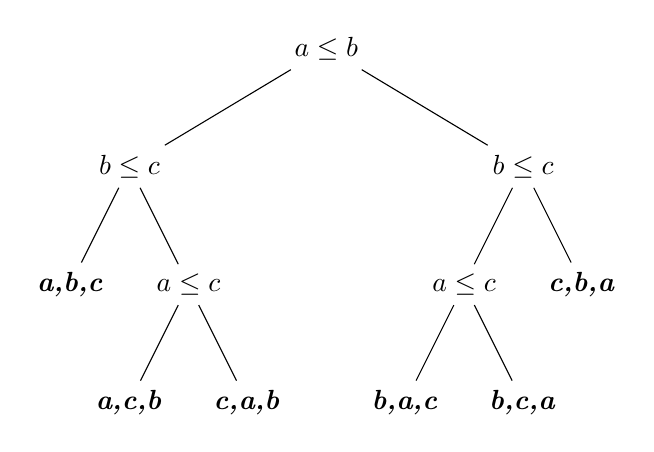
\begin{tikzpicture}[level distance=1.5cm,
  level 1/.style={sibling distance=5cm},
  level 2/.style={sibling distance=1.5cm},
  level 3/.style={sibling distance=1.5cm}]
  \node {$a \leq b$}
    child {node {$b \leq c$}
        child {node {\textbf{\textit{a,b,c}}}}
        child {node {$a \leq c$} {
          child {node {\textbf{\textit{a,c,b}}}}
          child {node {\textbf{\textit{c,a,b}}}}
      }}
    }
    child {node {$b \leq c$}
        child {node {$a \leq c$} {
          child {node {\textbf{\textit{b,a,c}}}}
          child {node {\textbf{\textit{b,c,a}}}}
      }}
          child {node {\textbf{\textit{c,b,a}}}}
    };
\end{tikzpicture}
\end{center}

Observe that the height or depth of the tree represents the amount of computations which must be performed.
Furthermore observe that the height of the tree is not the same for every root,
for the ordering \textbf{\textit{b,a,c}} we have height three
and for \textbf{\textit{a,b,c}} we have height two.
This is because we can prune some branches due to the transitive property of $\leq$,
given $a \leq b$ and $b \leq c$ we also know that $a \leq c$ is true.
Thus we do not need to compute $a \leq c$.
Conversely given $a \leq b$ and $c \leq b$ we \textbf{do not know} that $a \leq c$ is true.
This is another computation we need to perform to have a correct ordering.
Obviously this tree is correct for $n = 3$, so we can say
the complexity lower bound for $n = 3$ is 3 computational steps.
This is because equipped with only comparison we can only go in one
of two directions after each computation (true or false),
and we must be able to produce all six possible orderings.

How do
How many branches can we prune?

Well for a three item set $(a,b,c)$ there exists precisely $!3 = 6$ orderings;
thus our decision tree 
or more generally there exists for an $n$ item set $!n$ orderings.
Because
$$\Omega(n log n)$$


\subsection{Algebraic computation trees: examples}
We can expand the decision tree model to something more powerful

Consider the problem of finding if a point is inside the unit circle
\begin{itemize}
    \item Input: a point $(x,y) \in \mathbb{R}^2$
    \item Output: yes iff $x^2 + y^2 \leq 1$
\end{itemize}
The complexity of this algorithm (the height of the tree) is 4, i.e., a constant.
This is quite natural since we assume that the size of the input is a constant.
\begin{center}
    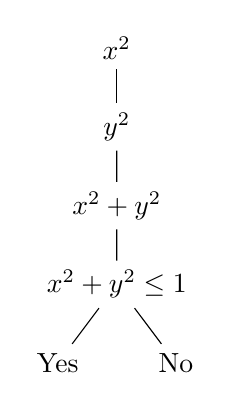
\begin{tikzpicture}[level distance=1cm,
  level 1/.style={sibling distance=2cm},
  level 2/.style={sibling distance=1.5cm},
  level 3/.style={sibling distance=1.5cm},
  level 4/.style={sibling distance=1.5cm},
  level 5/.style={sibling distance=1.5cm}]
  \node {$x^2$}
        child {node {$y^2$}
        child {node {$x^2 + y^2$}
        child {node {$x^2 + y^2 \leq 1$}
            child {node {Yes}}
            child {node {No}}
            }}
        };
\end{tikzpicture}
\end{center}

To further generalise our algebraic computation trees,
we will say that every node, except leaves, have three children.
The children correspond to the computation being
\begin{enumerate}
    \item $(= 0)$
    \item $(< 0)$
    \item $(> 0)$
\end{enumerate}
In the example below for the sake of space and brevity we don't show all the different branches,
simply because we never make any changes to our computation dependent on the result;
that is until the very end where we use it for our yes or no result.
This tree, were it completed, would have $3^4 = 81$ nodes,
much more than our previous tree.
However observe that the height remains unchanged at four,
thus the complexity is the same.

\begin{center}
    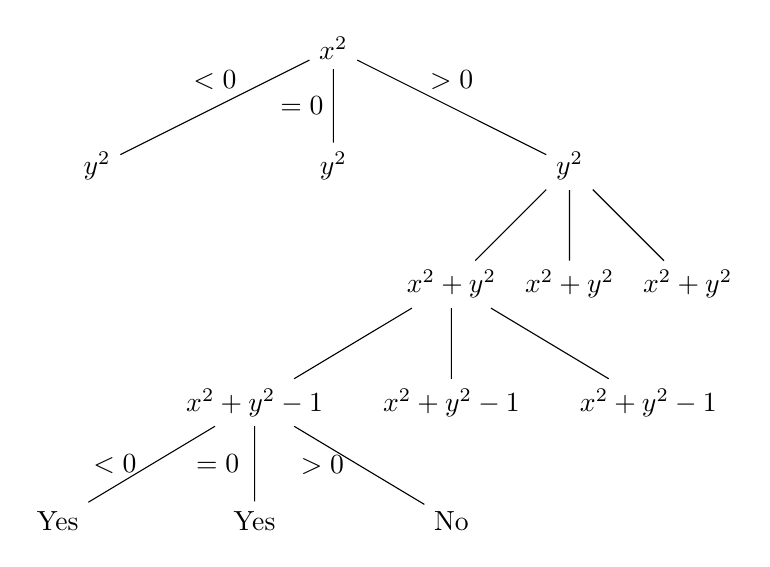
\begin{tikzpicture}[level distance=1.5cm,
  level 1/.style={sibling distance=3cm},
  level 2/.style={sibling distance=1.5cm},
  level 3/.style={sibling distance=2.5cm},
  level 4/.style={sibling distance=2.5cm}]
    \node {$x^2$}
            child {node {$y^2$} edge from parent node[left,above=3pt] {$< 0$}
            }
            child {node {$y^2$} edge from parent node[left] {$= 0$}
            }
            child {node {$y^2$}
                child { node {$x^2 + y^2$} 
                    child { node {$x^2 + y^2 - 1$} 
                        child { node {Yes} edge from parent node[left=2pt] {$< 0$}}
                        child { node {Yes} edge from parent node[left=2pt] {$= 0$}}
                        child { node {No}  edge from parent node[left=2pt] {$> 0$}}
                    }
                    child { node {$x^2 + y^2 - 1$} }
                    child { node {$x^2 + y^2 - 1$} }
                }
                child { node {$x^2 + y^2$} }
                child { node {$x^2 + y^2$} }
            edge from parent node[left,above=3pt] {$> 0$} }
       ;
\end{tikzpicture}
\end{center}

\begin{example}
    One can generalise this example from membership of the unit circle to membership
    of the $n$ dimensional unit ball.
    Simply calculate
    $$1 \leq \sum_{i=1}^{n} x_i^2$$
    You calculate $x_i^2$ for the $i$-th dimension and add it to the running total;
    this takes $2n$ steps.
    In case $n = 2$ we get complexity four as our computation tree showed.
\end{example}

\subsection{Algebraic computation trees: definition}
\begin{definition}
    A subset $S \subset R^n$ is called \textit{(basic) semi-algebraic} if it is defined by
    $$\{P_1(x_1,\dots x_n) = 0,\dots P_n\}
    \cup
    \{Q_1(x_1,\dots x_n) > 0,\dots Q_m\}$$
    where $P_i$ and $Q_j$ are polynomials in $n$ variables
    i.e., S is a set of all solutions of a system of equations and strict inequalities.
\end{definition}

Algebraic computation tree $T$ in variables $x_1,\dots x_n$
is a tree with the root $v_0$ such that to every vertex $v$ (except leaves)
is an arithmetic operation (addition, subtraction or multiplication) 
and a polynomial $f_v$ is attached.

For example $f_3 = f_1 + f_2$ where $f_3$ is the new polynomial;
more precisely in our previous example membership of the unit circle
we have
$$f_1 = x^2 \quad f_2 = y^2 \quad f_3 = x^2 + y^2$$
$$f_4 = f_3 - 1 = x^2 + y^2 - 1$$

Let $v_0, v_1,\dots, v_\omega$ be the sequence of vertices
along the (unique) branch leading from the root $v_0$ to $v_\omega$.
An arithmetic operation at $v_i$ is performed on a pair from
$$\{x_1,\dots x_n\} \cup \{f_0\dots f_{i - 1}\}$$
and the result is at $f_i$.
Note that every $v$ has exactly three children
$$(> 0, = 0, < 0)$$

Let $*_i \in \{>0,=0,<0\}$ for $0 \leq i < \omega$ be the sign of $f_{v_i}$,
One can assign the semi-algebraic set $U_\omega$ to $v_\omega$
$$U_\omega = \{f_0*_00,f_1*_10\dots f_{\omega - 1} *_{\omega - 1}0\}$$

To each leaf $\omega$ of $T$ an output Yes or No is assigned.
We call $U_\omega$ an accepting set if the leaf $\omega$ has the output Yes assigned.
We say that T tests the membership to the union of all accepting sets.

The computation process works as follows.
A specific point $x \in \mathbb{R}^n$ is taken as an input.
Then the value $f_{v_0}(x)$ is computed and the sign of this value is determined.
According to the sign, the algorithm goes to the corresponding child $v_1$ of $v_0$.
If the process eventually arrives to a Yes-vertex, then $x$ belongs to an accepting set,
and, therefore, to the union of all accepting sets.

\subsection{Distinctness problem: upper bound}
\begin{itemize}
    \item \textbf{Input:} $(x_0, x_1,\dots x_n) \in \mathbb{R}^n$
    \item \textbf{Output:} Yes iff $\forall\ i,j$ where $0 \leq i,j \leq n, i \neq j$ we have $x_i \neq x_j$
\end{itemize}
An immediate solution for this problem is to sort the numbers $(x_0, x_1,\dots x_n)$
then compare pairwise neighbours for equivalence; this has complexity $O(nlogn)$.
It is clear that this algorithm can be represented in a form of algebraic computation tree
of the height $O(nlogn)$ (compare with sorting).
We are going to develop a general method for proving lower complexity bounds for algebraic computation trees,
and will apply this method to prove the $\Omega(nlogn)$ lower bound for Distinctness.
Unlike the very elementary proof of $\Omega(nlogn)$ for sorting,
for Distinctness no elementary proof is known.

\subsection{Connected components of semialgebraic sets}
Informally, a finite union $W$ of semialgebraic sets is called connected
if for every $x, y \in W$ there is a “continuous” curve in $W$ containing both $x$ and $y$.
A formal definition can be found in textbooks on topology.

\begin{definition}
    Any maximal (with respect to the set-theoretical inclusion) connected subset of W is called connected component of W.
\end{definition}

\begin{theorem}
    Every finite union W of semialgebraic sets can be uniquely represented as a union of a finite number of its connected components:
    $$W = \bigcup\limits_{1\leq i \leq k} W_i$$
    which are finite unions of semialgebraic sets.
\end{theorem}

\begin{example}
    Consider these examples
    \begin{enumerate}
        \item The union of open intervals $W = (0, 1) \cup (2, 3) \subset R$ is \textbf{not} connected.
            Intervals $(0, 1)$ and $(2, 3)$ are connected components of W .
        \item The union $W = (0, 1) \cup (1, 2)$ is not connected with $(0, 1),\ (1, 2)$ being $W$’s connected components.
        \item The union $W = (0, 1) \cup 1 \cup (1, 2) = (0, 2)$ is connected and is its own unique connected component.
        \item The semialgebraic set $W = \{X \neq Y \} \in R^2$
            (which also can be written in the form $W = \{X^2 − 2XY + Y^2 > 0\}$)
            is not connected and has two connected components: $\{X − Y > 0\}$ and $\{Y − X > 0\}$.
    \end{enumerate}
\end{example}

\begin{theorem}
    Projection of a connected set $W \subset R^{n+m}$ on a coordinate subspace $R^n$ is also connected.
\end{theorem}

\subsection{Lower bound for membership to a semialgebraic set: decision computation trees}
\subsection{Thom-Milnor’s bound}
\subsection{Lower bound for membership to a semialgebraic set: algebraic computation trees}
\subsection{Distinctness problem: lower bound}
